\documentclass[]{beamer}
% \geometry{papersize={16cm,9.60cm}}
\usepackage{etex}
\usepackage{amsmath}
\usepackage{tikz}
\usepackage{multimedia}
\usetheme{Boadilla}
\usepackage{graphicx}
\usepackage{url}

%\usepackage{inputenc}

% \mode<presentation>
% {
%   \usetheme{default}
%   \setbeamercovered{transparent}
% }


% {\vskip5pt}

%% customize layout, bullet points navigation toolbar
\setbeamertemplate{navigation symbols}{}%remove navigation symbols
\setbeamertemplate{enumerate items}[default]
\setbeamertemplate{navigation symbols}{}
\setbeamertemplate{itemize items}[circle]
\setbeamercolor{enumerate item}{fg=black}

\setbeamertemplate{footline}{}
\setbeamersize{text margin left = 2.0em}
\setbeamersize{text margin right = 2.0em}


\usepackage{times}
\usepackage[T1]{fontenc}

% Or whatever. Note that the encoding and the font should match. If T1
% does not look nice, try deleting the line with the fontenc.

\setbeamertemplate{navigation symbols}{}

\title{ Cognitive (Neuro) Psychology }
\subtitle{VII. Perceiving Motion}
\author{ Marianne Maertens }
\institute[TU Berlin]{Technische Universit\"at Berlin}
\date{September 2016}

\begin{document}
\setbeamertemplate{enumerate items}[default]
\setbeamertemplate{headline}

\frame{\titlepage}

\AtBeginSection[]
{
  \begin{frame}<beamer>
    \frametitle{Layout}
    \tableofcontents[currentsection]
  \end{frame}
}



\begin{frame}
 \frametitle{Objectives}
\begin{overlayarea}{110mm}{70mm}
 basic knowledge in
\begin{itemize}
  \item Cognitive (Neuro) \textbf{Psychology}
  \item Experimental Methods
\end{itemize}

\vspace{5mm}
\only<2->{
\begin{itemize}
 \item[$\Rightarrow$] What kind of questions are addressed in the discipline?
 \item[$\Rightarrow$] How are these questions being addressed?
 \item[$\Rightarrow$] Be able to comprehend and evaluate literature and work done in the field.
\end{itemize}
}
\end{overlayarea}
\end{frame}

\begin{frame}
 \frametitle{Topics \& Structure}
\includegraphics<1>[width=120mm]{figs/l7/timetable.pdf} 
\end{frame}


\begin{frame}
 \frametitle{Philosophy}
\begin{overlayarea}{110mm}{50mm}
Challenge: block course!! \\
\vspace{5mm}
\only<2->{
 \begin{itemize}
  \item alternation between instruction and individual studies
  \item active involvement of participants
  \item some topics in depth instead of broad coverage
  \item exam: indicate the degree of retention of material - MC 
  \item[]
  \item<3->[?] Comments, Questions?
 \end{itemize}
}
\end{overlayarea}
\end{frame}


\begin{frame}
\begin{center}
 \begin{LARGE}
What happened so far? 
\end{LARGE}
 \end{center}
\end{frame}


\begin{frame}{Recap}
 \begin{overlayarea}{110mm}{70mm}
  \begin{columns}[T]
   \begin{column}{60mm}
    \begin{itemize}
     \item Experimental methodology
    \begin{itemize}
     \item<1-> Hypothesis, experimental design, etc.
     \item<2-> Psychophysics, thresholds, sensitivity
     \item<3-> Measuring appearance 
    \end{itemize}
   \item<4-> Visual information processing
    \begin{itemize}
     \item<4-> Properties of visual neurons, orientation selectivity, spatial frequency selectivity, ...
     \item<5-> Visual functions, orientation discrimination, acuity, ...
     \item<6-> Object recognition
    \end{itemize}
   \end{itemize}
   \end{column}

   \begin{column}{50mm}
    \begin{center}
    \includegraphics<1>[width=50mm]{../../../figures/huber_hypothesis.png}
   \includegraphics<2>[width=40mm]{../../../figures/muller_lyer_pmf_pse.png}
   \includegraphics<3>[width=40mm]{figs/l6/knoblauch_scaling98.png}
   \includegraphics<4>[width=40mm]{figs/l5/ventral_pathways.png}
   \includegraphics<5>[width=40mm]{figs/l3/csf_demo.png}
   \includegraphics<6>[width=50mm]{figs/l5/T_junctions.png}
   \end{center}
  \end{column}
  \end{columns}
 \end{overlayarea}
\end{frame}



\begin{frame}
 \frametitle{What do you see?}
\begin{overlayarea}{130mm}{80mm}
 \begin{center}
\includegraphics<1>[width=50mm]{figs/l7/ladybug_1.png}
\includegraphics<2->[width=50mm]{figs/l7/ladybug_2.png}
 \end{center}
\only<3->{\textcolor{blue}{Motion} is a change in location over time.}
\end{overlayarea}
 \end{frame}

\begin{frame}
 \frametitle{Overview}
\begin{itemize}[<+->]
  \setlength{\itemsep}{5pt}
 \item How is motion computed in the brain?
 \item What is difficult in motion perception?
 \item Functions of motion perception
 \item Eye movements
\end{itemize}
\end{frame}


\begin{frame}
 \frametitle{The computation of motion in the brain}
\begin{overlayarea}{130mm}{70mm}
Motion is a change in position over time
 \begin{center}
\includegraphics<1>[width=70mm]{figs/l7/ladybug.png}
 \end{center}
How would you build a motion detector?
\end{overlayarea}
\end{frame}

\begin{frame}
\frametitle{The computation of motion in the brain}
\begin{overlayarea}{110mm}{80mm}
\begin{itemize}
 \item<1-> start with two adjacent receptors, A and B
 \item<2->[$\rightarrow$] registers change in position
 \item<3-> simply adding inputs $\rightarrow$ not motion-selective
 \item<4-> \textbf{D}elay cell, fast adapting 
 \item<5-> \textbf{X} - multiplies D with receptor B's response
\end{itemize}

 \begin{center}
\includegraphics<1-2>[width=70mm]{figs/l7/reichardt_detector_2cells_1.png}
\includegraphics<3>[width=70mm]{figs/l7/reichardt_detector_2cells_0.png}
\includegraphics<4->[width=70mm]{figs/l7/reichardt_detector_2cells.png}
 \end{center}
\end{overlayarea}
\end{frame}


\begin{frame}
 \frametitle{"Bug`` motion detector}
\begin{overlayarea}{130mm}{70mm}
first described by Werner Reichardt (1950)
 \begin{center}
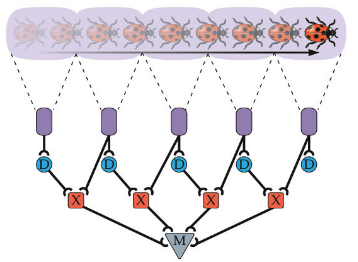
\includegraphics[width=60mm]{figs/l7/reichardt_detector_manycells.png}
 \end{center}
\only<2->{
\begin{itemize}
 \item direction-selective
 \item tuned to velocity 
 \item fast adaptation prevents response to large objects
\end{itemize}
}
\end{overlayarea}
\end{frame}



\begin{frame}
\begin{block}{Activity}
Explore the motion detection circuit with the activity on the following webpage \url{http://sites.sinauer.com/wolfe4e/wa08.01.html}
\end{block}
\end{frame}



\begin{frame}
 \frametitle{Apparent motion}
 \begin{overlayarea}{110mm}{80mm}
\begin{itemize}
   \item Reichardt detector does not require continuous motion,
   \item[$\rightarrow$]\textcolor{blue}{prediction:} responds equally to object that appears in A's receptive field, disappears and reappears in B's receptive field
\end{itemize}

\begin{columns}[T]
 \begin{column}{40mm}
\includegraphics<1->[width=30mm]{figs/l7/reichardt_detector_single.png}
 \end{column}

 \begin{column}{40mm}
\begin{center}
\includegraphics<2>[width=40mm]{figs/l7/daumenkino_daffy_1.png} 
\includegraphics<3>[width=40mm]{figs/l7/daumenkino_daffy_2.png} 
\includegraphics<4>[width=40mm]{figs/l7/daumenkino_daffy_3.png} 
\includegraphics<5>[width=40mm]{figs/l7/daumenkino_daffy_4.png} 
\end{center}
\end{column}
\end{columns}
\end{overlayarea}
\end{frame}


\begin{frame}
\frametitle{Apparent motion}
 \begin{overlayarea}{110mm}{80mm}
 \begin{itemize}
 \item[=] illusory impression of smooth motion resulting from rapid alternation of objects that appear in different locations in rapid succession
 \item stop-motion, phi-phenomenon
\end{itemize}
\begin{center}
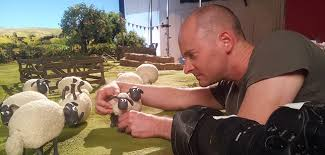
\includegraphics[width=70mm]{figs/l7/filming_shaun2.jpg} 
\end{center}

\only<2-> {\vspace{3mm}\textcolor{gray}{Web Activity 8.2}}
\end{overlayarea}
\end{frame}

\begin{frame}
 \frametitle{The correspondence problem}
\begin{overlayarea}{110mm}{80mm}
 \begin{columns}[T]
 \begin{column}{40mm}
\includegraphics<1->[width=35mm]{figs/l7/correspondence_1.png}
 \end{column}

 \begin{column}{40mm}
\includegraphics<1->[width=35mm]{figs/l7/correspondence_2.png} 
\end{column}
\end{columns}

\vspace{3mm}
How does the visual system know which circles in frame 2 correspond to which circles in frame 1?
\begin{center}
\includegraphics<2>[width=40mm]{figs/l7/correspondence_3.png} 
\end{center}
\end{overlayarea}
\end{frame}

\begin{frame}
 \frametitle{The aperture problem}
\begin{overlayarea}{120mm}{70mm}
when a moving object is viewed through an aperture, the direction of motion of a local part of the object may be ambiguous 
\begin{center}
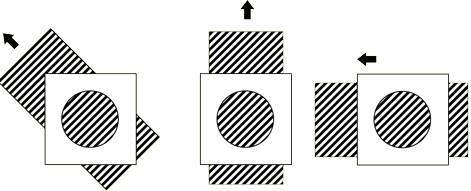
\includegraphics[width=80mm]{figs/l7/aperture.png} 
\end{center}

\only<2->{
\begin{itemize}
 \item Why is such an artificial situation relevant at all?
 \item<3->[$\rightarrow$] every V1 cell sees the world through a small aperture
\end{itemize}
}
\end{overlayarea}
\end{frame}


\begin{frame}
 \frametitle{Local vs. global motion}
\begin{overlayarea}{110mm}{70mm}
\begin{columns}[T]
\begin{column}{70mm}
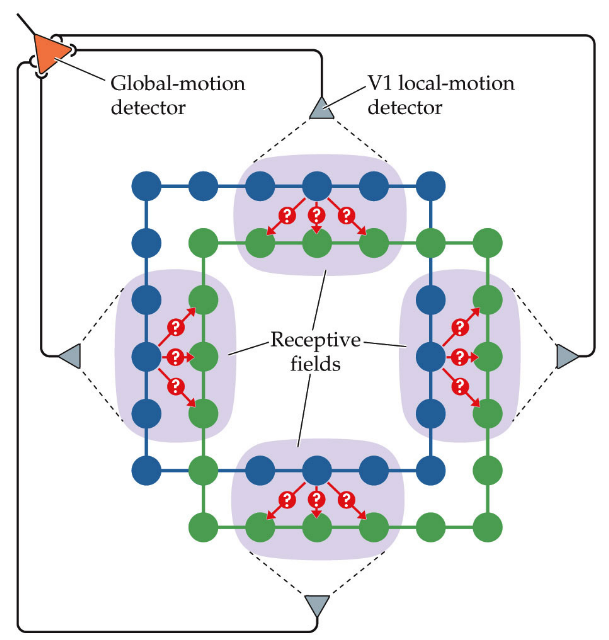
\includegraphics[width=70mm]{figs/l7/global_motion.png} 
\end{column}

\begin{column}{50mm}
\only<2->{
\begin{itemize}
 \item none of the V1 cells can tell with certainty which visual elements correspond to one another when an object moves
 \item<3->[$\rightarrow$] have another set of neurons 'listen' to the V1 neurons and integrate the potentially conflicting signals 
\end{itemize}
}
\end{column}
 \end{columns}
\end{overlayarea}
\end{frame}

\begin{frame}
 \frametitle{Where in the brain are global motion detectors?}
\begin{overlayarea}{110mm}{80mm}
\begin{center}
\includegraphics<1>[width=90mm]{figs/l7/cortical_pathways_motion.png} 
\includegraphics<2->[width=70mm]{figs/l7/MT_brain.png}  
\end{center}
\only<2->{
\begin{itemize}
 \item area MT in non-human primates - middle temporal area
 \item human equivalent of MT localized with fMRI MT+/V5
 \item<3-> MT cells are selective for motions in one particular direction
 \item<4->[$\rightarrow$] \textit{Are MT cells global or local motion detectors?}
\end{itemize}
}
\end{overlayarea}
\end{frame}


\begin{frame}
 \frametitle{Newsome and Pare (1988) paradigm}
\begin{overlayarea}{110mm}{70mm}
\begin{center}
\includegraphics<1->[width=90mm]{figs/l7/newsome_pare.png} 
\end{center}

\begin{itemize}
 \item monkeys were trained in motion discrimination in correlated dot displays
 \item<2-> no single dot sufficient to signal overall direction of motion
 \item<2->[$\rightarrow$] to detect correlated motion direction neuron must integrate information from many locations
\end{itemize}
\end{overlayarea}
\end{frame}


\begin{frame}
 \frametitle{Newsome and Pare (1988) paradigm}
\begin{overlayarea}{110mm}{70mm}
\begin{center}
\includegraphics<1->[width=90mm]{figs/l7/newsome_pare.png} 
\end{center}

\begin{itemize}
 \item after training monkeys recognized motion direction with only 2-3\% coherent dots
 \item<2-> experimental \textcolor{blue}{lesion} of area MT
 \item<3->[$\Rightarrow$] following surgery discrimination thresholds were 10 times as high: 20\% coherent dots
 \item<3->[$\Rightarrow$] ability to discriminate orientation of stationary patterns was generally unimpaired
\end{itemize}
\end{overlayarea}
\end{frame}

\begin{frame}
 \frametitle{Salzman, Britten \& Newsome, 1990}
 \begin{itemize}
  \item lesions may be incomplete or may affect other structures
  \item[]
  \item<2-> new group of monkeys was trained on motion discrimination
  \item<2-> recording of neurons to find groups of neurons that responded to one particular direction of motion
 \item[]
 \item<3-> stimulation with leftward motion while electrically stimulating neurons that respond to rightward motion
 \item<3->[?]
 \item<4-> monkeys reported motion in the stimulated neuron's preferred direction  
 \end{itemize}
\end{frame}

\begin{frame}
 \frametitle{Motion aftereffects (MAE)}
\begin{overlayarea}{110mm}{70mm}
 \begin{itemize}
  \item converging evidence for motion perception in humans?
 \item<2-> MAE: illusion of motion of a stationary object that occurs after prolonged exposure to a moving object
 \end{itemize}

\only<3->{
\begin{block}{Activity}
Explore the motion aftereffect with the activity on the following webpage \url{http://sites.sinauer.com/wolfe4e/wa08.04.html}
\begin{itemize}
 \item What happens when you adapt to downward motion and then look at something moving horizontally? Make a prediction and then test your hypothesis!
 \item Adapt for 15 s ro rightward motion with your right eye open and left eye closed. After adaptation quickly switch your eyes when looking at the test. 
\end{itemize}

 \end{block}
}
\end{overlayarea}
\end{frame}


\begin{frame}
 \frametitle{Functions of motion perception: Object identification}
\begin{center}
\includegraphics<1->[width=90mm]{figs/l7/biomotionlab.png} 
\end{center}

\url{https://www.biomotionlab.ca/Demos/BMLwalker.html}
\end{frame}

\begin{frame}
\frametitle{Functions of motion perception: Avoid collision}
\begin{overlayarea}{110mm}{70mm}
How do we estimate time to collision (TTC) of an approaching object?\begin{columns}[T]
\begin{column}{70mm}
\begin{itemize}
 \item small cricket ball bounces off the ground 3m away from player moves with constant rate of 15$\frac{m}{s}$
 \item $TTC = \frac{distance}{rate} = \frac{3}{15} = 0.2s$
 \item humans better at judging TTC than at judging distances
 \item[$\Rightarrow$] $\tau = \frac{\theta}{\dot{\theta}}$, heuristic
  \item[] $\theta$ - visual angle of object at any moment
  \item[] $\dot{\theta}$ - rate of change of visual angle 
\end{itemize}
\end{column}

\begin{column}{50mm}
\begin{center}
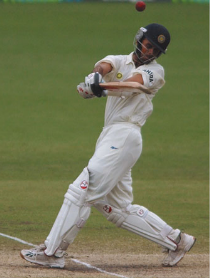
\includegraphics[width=30mm]{figs/l7/ttc.png} 
\end{center}
\end{column}
 \end{columns}
\end{overlayarea}
\end{frame}


\begin{frame}
\frametitle{Eye movements - physiology}
\begin{overlayarea}{110mm}{70mm}
 \begin{center}
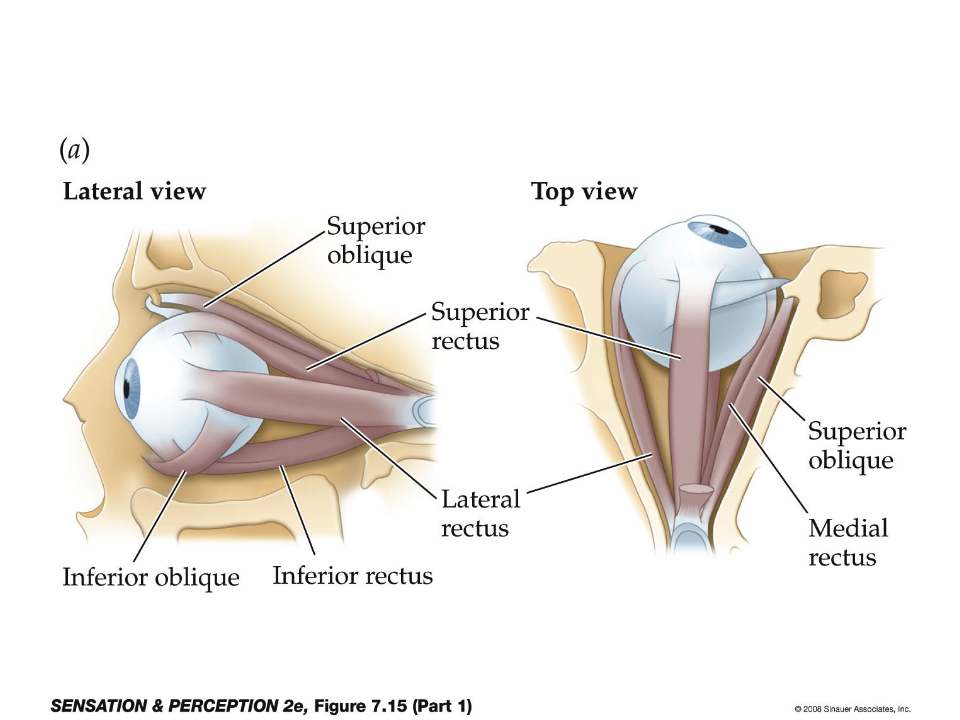
\includegraphics[width=70mm]{figs/l7/six_eye_muscles.png} 
\end{center}
\begin{itemize}
 \item eye muscles controlled by extensive network of structures in the brain
\end{itemize}

\end{overlayarea}
\end{frame}



\begin{frame}
\frametitle{Eye movements - physiology}
\begin{overlayarea}{110mm}{80mm}
 \begin{center}
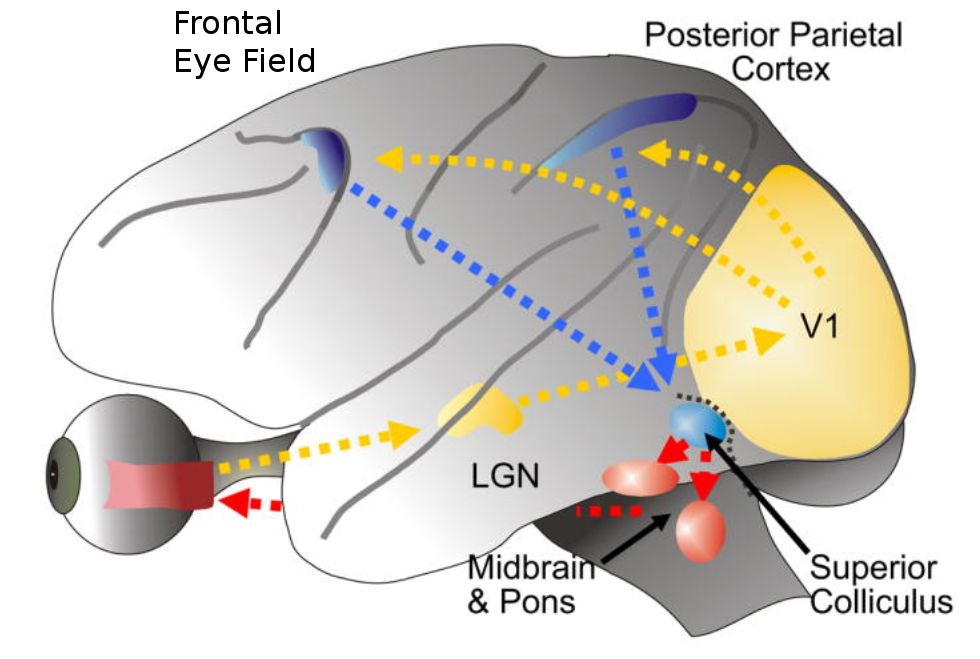
\includegraphics[width=70mm]{figs/l7/wurtz_em_brain.png} 
\end{center}

How to probe the role of brain structures in control of eye movements?
\begin{itemize}
 \item<2->[$\rightarrow$] stimulation of neurons and observation of eye movements
\end{itemize}
\only<2->{\textbf{superior colliculus} - eyes move by specific amount in specific direction\\}
\only<3->{\textbf{frontal eye fields} - eyes move toward specific location}
\end{overlayarea}
\end{frame}


\begin{frame}
\frametitle{Types of eye movements}
\begin{overlayarea}{110mm}{80mm}
 \begin{itemize}
  \item[] \textbf{smooth pursuit} - eye moves smoothly to follow a moving object
  \item[] \textbf{vergence} - inward or outward rotation on the eye to focus on near or far object
  \item[] \textbf{saccades} - eye rapidly changes location from one fixation position to the next
 \begin{itemize}
 \item[] \textbf{microsaccades} - involuntary small eye movement
 \end{itemize}
 \end{itemize}

 \begin{center}
\includegraphics<2->[width=60mm]{figs/l7/classic_scan_path.png} 
\end{center}
\end{overlayarea}
\end{frame}


\begin{frame}
 \frametitle{Eye movements}
\begin{overlayarea}{110mm}{80mm}
\begin{center}
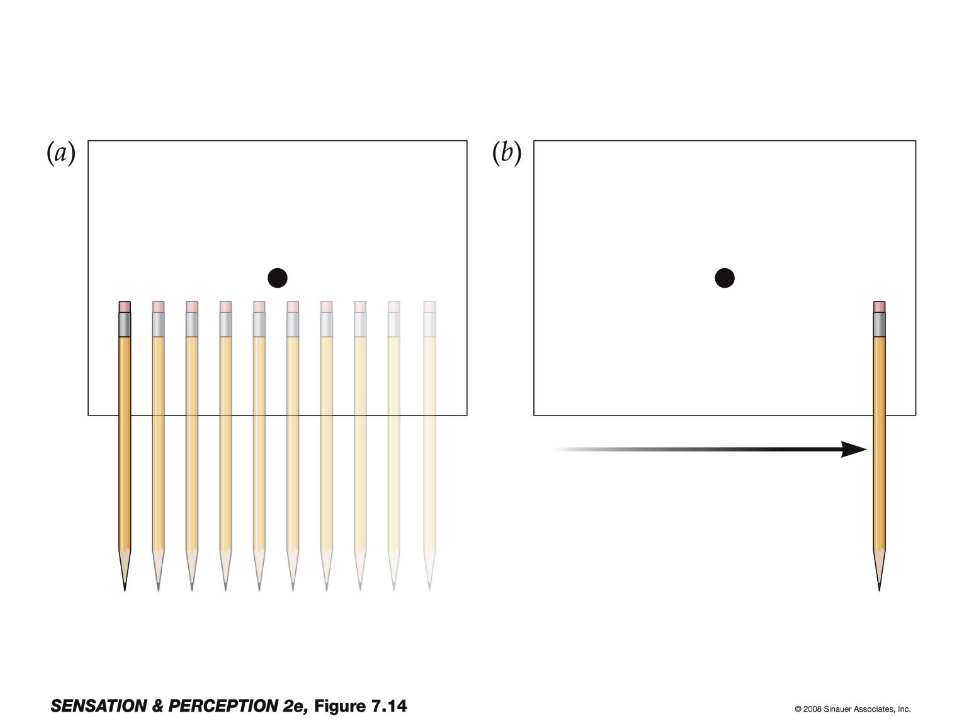
\includegraphics[width=70mm]{figs/l7/eye_movement_demo.png} 
\end{center}
\begin{enumerate}[(a)]
 \item close one eye, focus on dot, move pencil from lower right to left
 \item start with pencil at bottom left, fixate eraser, track it while moving the pencil to the right
\end{enumerate}

\only<2->{
Image of dot (b) and of pencil (a) make the same journey on the retina - one is perceived as moving the other not. Why?
}
\end{overlayarea}
\end{frame}


\begin{frame}
\frametitle{Saccadic Suppression and the Efference Copy}
\begin{overlayarea}{120mm}{80mm}
 How do we discriminate motion across the retina that is due to eye movements from motion due to object movement?\\ \vspace{2mm}
% Demo: ''jiggle`` the eyeball
 \begin{center}
\includegraphics<2->[width=70mm]{figs/l7/efference_copy.png} 
\end{center}
 
\only<3->{\textbf{Saccadic suppression} - reduction in sensitivity during eye movements}
\end{overlayarea}
\end{frame}


\begin{frame}
 \frametitle{Summary}
\begin{itemize}
\setlength{\itemsep}{5pt}
 \item Motion is a primary visual dimension like color or orientation
 \item Motion information helps to determine where objects are going and how we move through the environment without being hit
 \item V1 neurons view the world through small windows leading to the aperture problem
 \item behavioral and physiological evidence suggests that area MT is involved in the perception of global motion
 \item it is still not understood how we perceive a stable world when the retinal image undergoes permanent changes due to eye movements
\end{itemize}
\end{frame}



\begin{frame}
 \frametitle{References}
\begin{small}
\begin{itemize}
 \item  Wolfe, J.M., Kluender, K.R. \& Levi, D.M. (2012).\textit{Sensation \& Perception}. Sinauer Associates: Sunderland, MA. 
\end{itemize}
\end{small}
\end{frame}


\end{document}